\section{Methodology}
% Description of your proposed methodology or approach
In this section, we display how effective image preprocessing and our docking procedure collectively lead to a plausible method to train our model without manual labeling, which would be required, for our case, in real-world applications. Our methodology includes data collection, data preprocessing, model training, inference, server integration, evaluation, and experimental setup.

\subsection{Data Collection}
We collect training data using a simulated environment created in a game engine \citep{hoster2024usinggameenginesmachine}. Our game engine of choice is Godot, a free and open source game engine. The environment consists of a robot, a data camera, the alignment target (target 1) and the docking station (target 2). The data camera is scripted so that it captures images of the environment from various angles. The target that the data camera focuses on during the data gathering process can either be the alignment target or the docking station. What is important is that, in our data preprocessing, we exclude images that don't have their respective target in them, as explained in the next section.

The data camera is not randomly moving, and then taking a picture. Rather, it moves right to left in a predefined amount of steps. At each step, the data camera looks at our target, and rotates a predefined angle horizontally. This is because each step has its own number of what we call rotational images, which are images that are taken at the position of the step, but horizontally rotated slightly each time. Once the data camera has reached the end of the row moving left, we can move forward to the next row, and repeat the process. We do this until we are close enough to the dock.
\begin{figure}
    \centering
    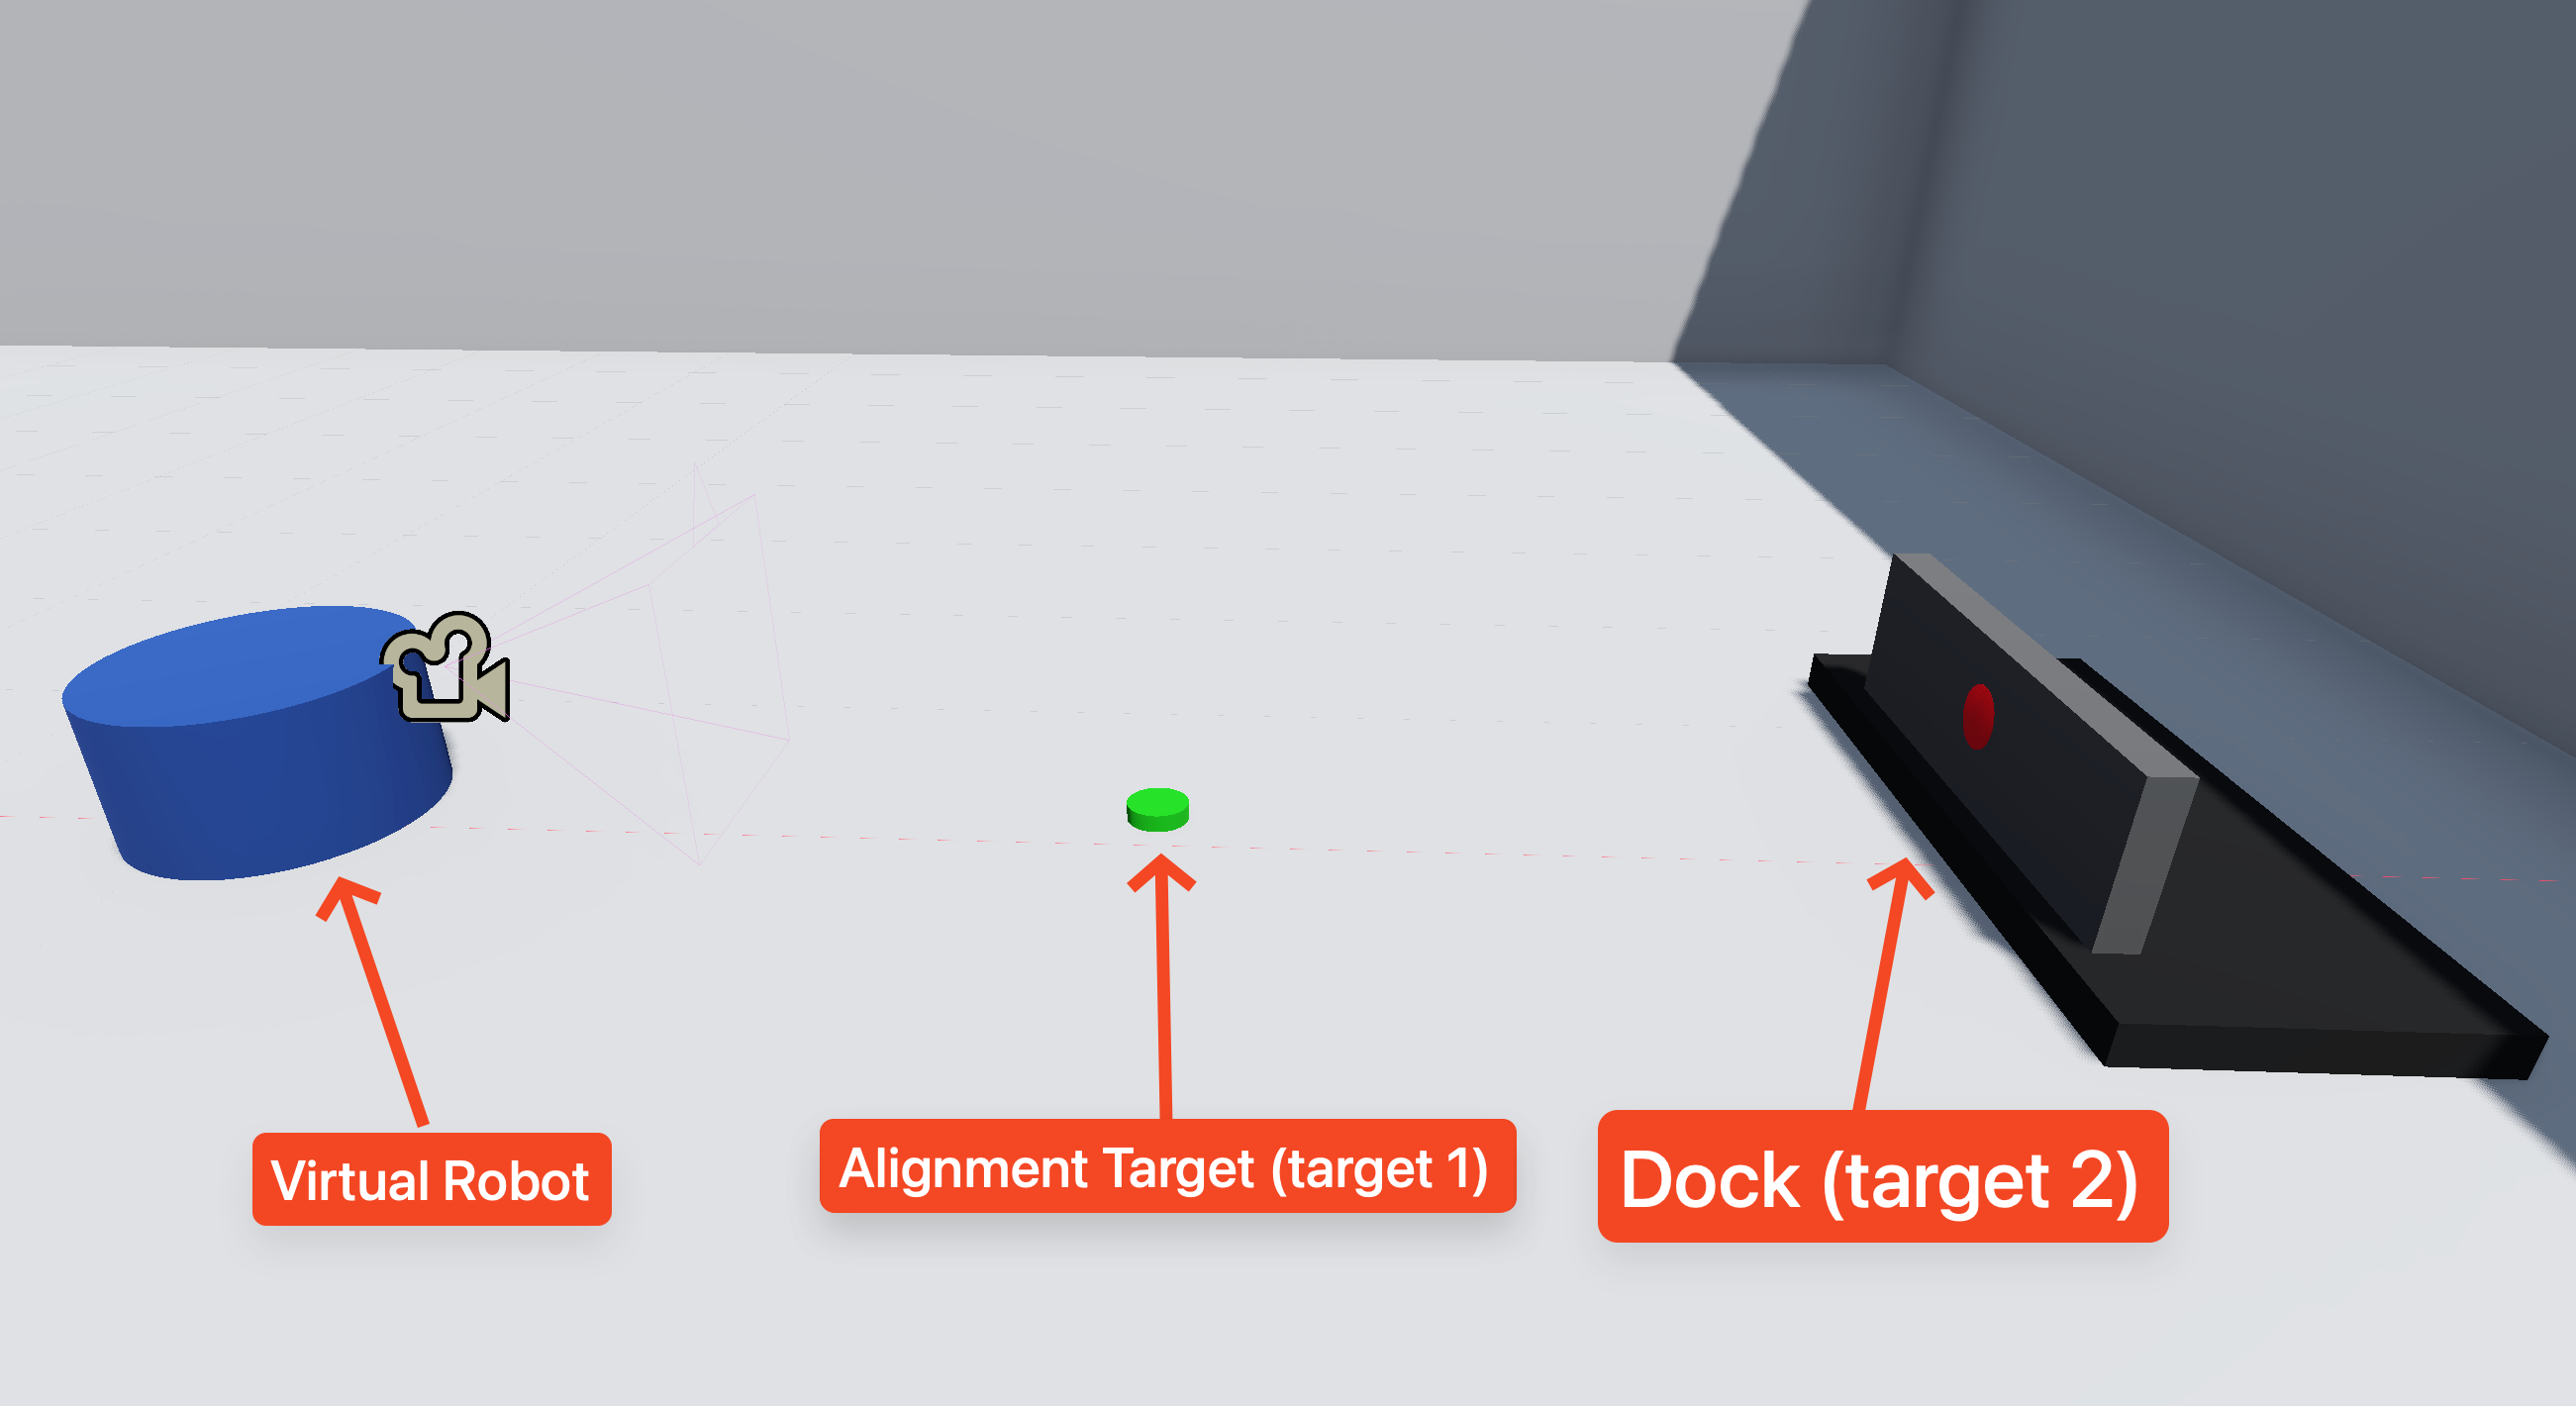
\includegraphics[width=\linewidth]{figures/src/virtual_world.png}
    \caption{
	    \textbf{Virtual world \& Labels} In our virtual world, we make targets 1 and 2 distinguishable from their surrounding environment by giving them a unique color.
    }
    \label{fig:virtual world}
\end{figure}


The reason we want to collect our data this way is because we want to make our data inclusive. With randomization, we don't know for sure if there will be images that are extremely similar, and we don't know if each angle is represented fairly. The diagram below shows what the data camera movement looks like from a bird's eye view.

\textbf{Data Camera Movement figure here}

\subsection{Data Preprocessing}
We preprocess the collected images in order to have a dataset of images and their corresponding target values. In order to do this, we use OpenCV to detect the targets. This is really only a viable option due to the fact that we chose unique colors for our targets that aren't present anywhere else in the virtual world. In real life, contour detection like this wouldn't work, and we would need to manually label where the targets are.

Contour detection returns a list of coordinates that outline a target. We, however, only want one coordinate. We can achieve this by approximating the center of the target, which can be done by taking the mean of both the \(x\) and the \(y\) values of the contour coordinates list.

\[
	\bar{x} = \frac{1}{n}\sum_{i=1}^{n} x_i ~\text{,} ~\bar{y} = \frac{1}{n}\sum_{i=1}^{n} y_i
\]
\textbf{Here we add two images, one showing the outline of the target, and one showing the center of the target. (like a before and after)}

Our data is then be sorted into two sets of data, one set specifically for the alignment target, and one specifically for the docking station. The reason we do this is because our custom models are not trained the same way YOLO models are trained, meaning we don't know if the object is actually in frame. So, if one target is in an image, it doesn't necessarily mean that the other one is as well. The two sets of data share images, but one set may have more or less images than the other. This is because at some angles, one target may be visible while the other is not. In our case, the set of data that has more images is the one where we focused the target on during data gathering in the Godot game engine, which was target 1 (the green target). 

\textbf{Here we add an image that includes the alignment target but not the docking target)}

This sorting of data for each model is done through OpenCV. If contour detection is not present for one of the targets, the image is not included in the dataset for the image not found. This applies to both targets in the same function, meaning, if no targets are found, the image is essentially discarded. Again, using OpenCV for these operations is highly possible because we are in a virtual environment where the colors of the targets are unique to themselves.

The sorting of data for the two separate models also means that each model may be performed differently. However, in our data collection, the difference in image amount was around 500 (\textbf{CHECK THIS NUMBER}). This is not a significant difference, and we can still train the models in very similar ways. The only difference is that the model that has less images may have a lower accuracy, which is where our custom data augmentation comes in.


\subsection{Model Training}
Near the end of this paper, we describe how our methodology can be implemented using a single YOLO model for object detection and prediction, all in one package. The reason why we have initially developed our project with custom models is because we more have flexibility regarding the architecture and performance of the models. By implementing the models using PyTorch, we can make lower level modifications to essentially see what the most conservative model is that can still perform well. This is important because we want to make sure that our model is as lightweight as possible. We don't want to have a model that is too heavy, because it will be running on a robot that has limited computational power.

Our training process is quite standard and is as follows:
\begin{enumerate}
    \item Load and preprocess the images using the `transforms` module from torchvision.
    \item Define the custom dataset class `TargetsDataset` to handle the input data.
    \item Instantiate the model, loss function (L1 Loss), and optimizer (Adam).
    \item Train the model over multiple epochs, applying custom image augmentation techniques to improve generalization.
\end{enumerate}

The first, second, and third steps in the list above are all standard ways to train a PyTorch model, or any basic deep learning model like the one we are creating. For the fourth step, the reason we need to apply custom image augmentation is because of coordinate predictions on the image. If we use the built-in method of image augmentation that PyTorch provides, the coordinates of the data will be off. The image is being transformed, but the coordinates are not. 

In order to solve this, we implement our own vertical flip augmentation, which returns the transformed image and the transformed coordinates. This way, the model can learn to predict the correct coordinates, even if the image is flipped. The reason we only need to implement a vertical flip is because, if we also implemented the horizontal flip, the data would have very similar looking images, as the flipped images would be almost identical to the images taken on the other side of the robot during data gathering.

\subsection{Inference}
For inference, we use the trained model to predict the next action based on a single input frame. The `predict` function takes an image as input, preprocesses it, and outputs the predicted target coordinates.

\subsection{Server Integration}
To facilitate real-time predictions, we can integrate the inference script with a Flask server, as shown in . The server receives images via POST requests, runs the inference, and returns the next action the virtual robot should take. This setup allows for seamless integration with other systems and real-time decision-making.

\subsection{Evaluation}
We evaluate the performance of our model using various metrics, including accuracy and loss values. The evaluation scripts are included in [tests/tests.py](tests/tests.py), which contain unit tests to ensure the correctness and robustness of our data processing and model training pipelines.

\subsection{Experimental Setup}
Our experimental setup involves running the training and inference scripts on a machine with a GPU to accelerate the deep learning computations. The models are saved in the [models](models) directory, and the results are analyzed and visualized using matplotlib.

\subsection{Conclusion}
Our methodology demonstrates a novel approach to robot docking using monocular vision and deep learning. By leveraging a simulated environment for data collection and a robust training pipeline, we achieve accurate and efficient docking without the need for additional sensors or reinforcement learning.
